\starthis\section[二维中心力场]{二维中心力场} \label{sec:05.05} % 
% \makebox[5em][s]{} % 短题目拉间距

在二维问题中,常用的坐标系有直角坐标$(x,y)$和平面极坐标$(\rho,\varphi)$,如图5 -5所示,它们的关系是
\begin{empheq}{align}
	x=\rho\cos\varphi,\quad y&=\rho\sin\varphi	\label{eq55.1}\\
	\rho=\sqrt{x^{2}+y^{2}},\quad \varphi&=\arctan\frac{y}{x}	\label{eq55.2}
\end{empheq}
粒子(质量$\mu$)受到二维中心力场作用时,势能$V$是径向距离$\rho$的函数,总能量算符可以表示成
\begin{empheq}{equation}\label{eq55.3}
	\hat{H}=\hat{T}+\hat{V}=-\frac{\hbar^{2}}{2\mu}\nabla^{2}+V(\rho)
\end{empheq}

\begin{wrapfigure}[8]{r}{6em}
	\centering
	\small
	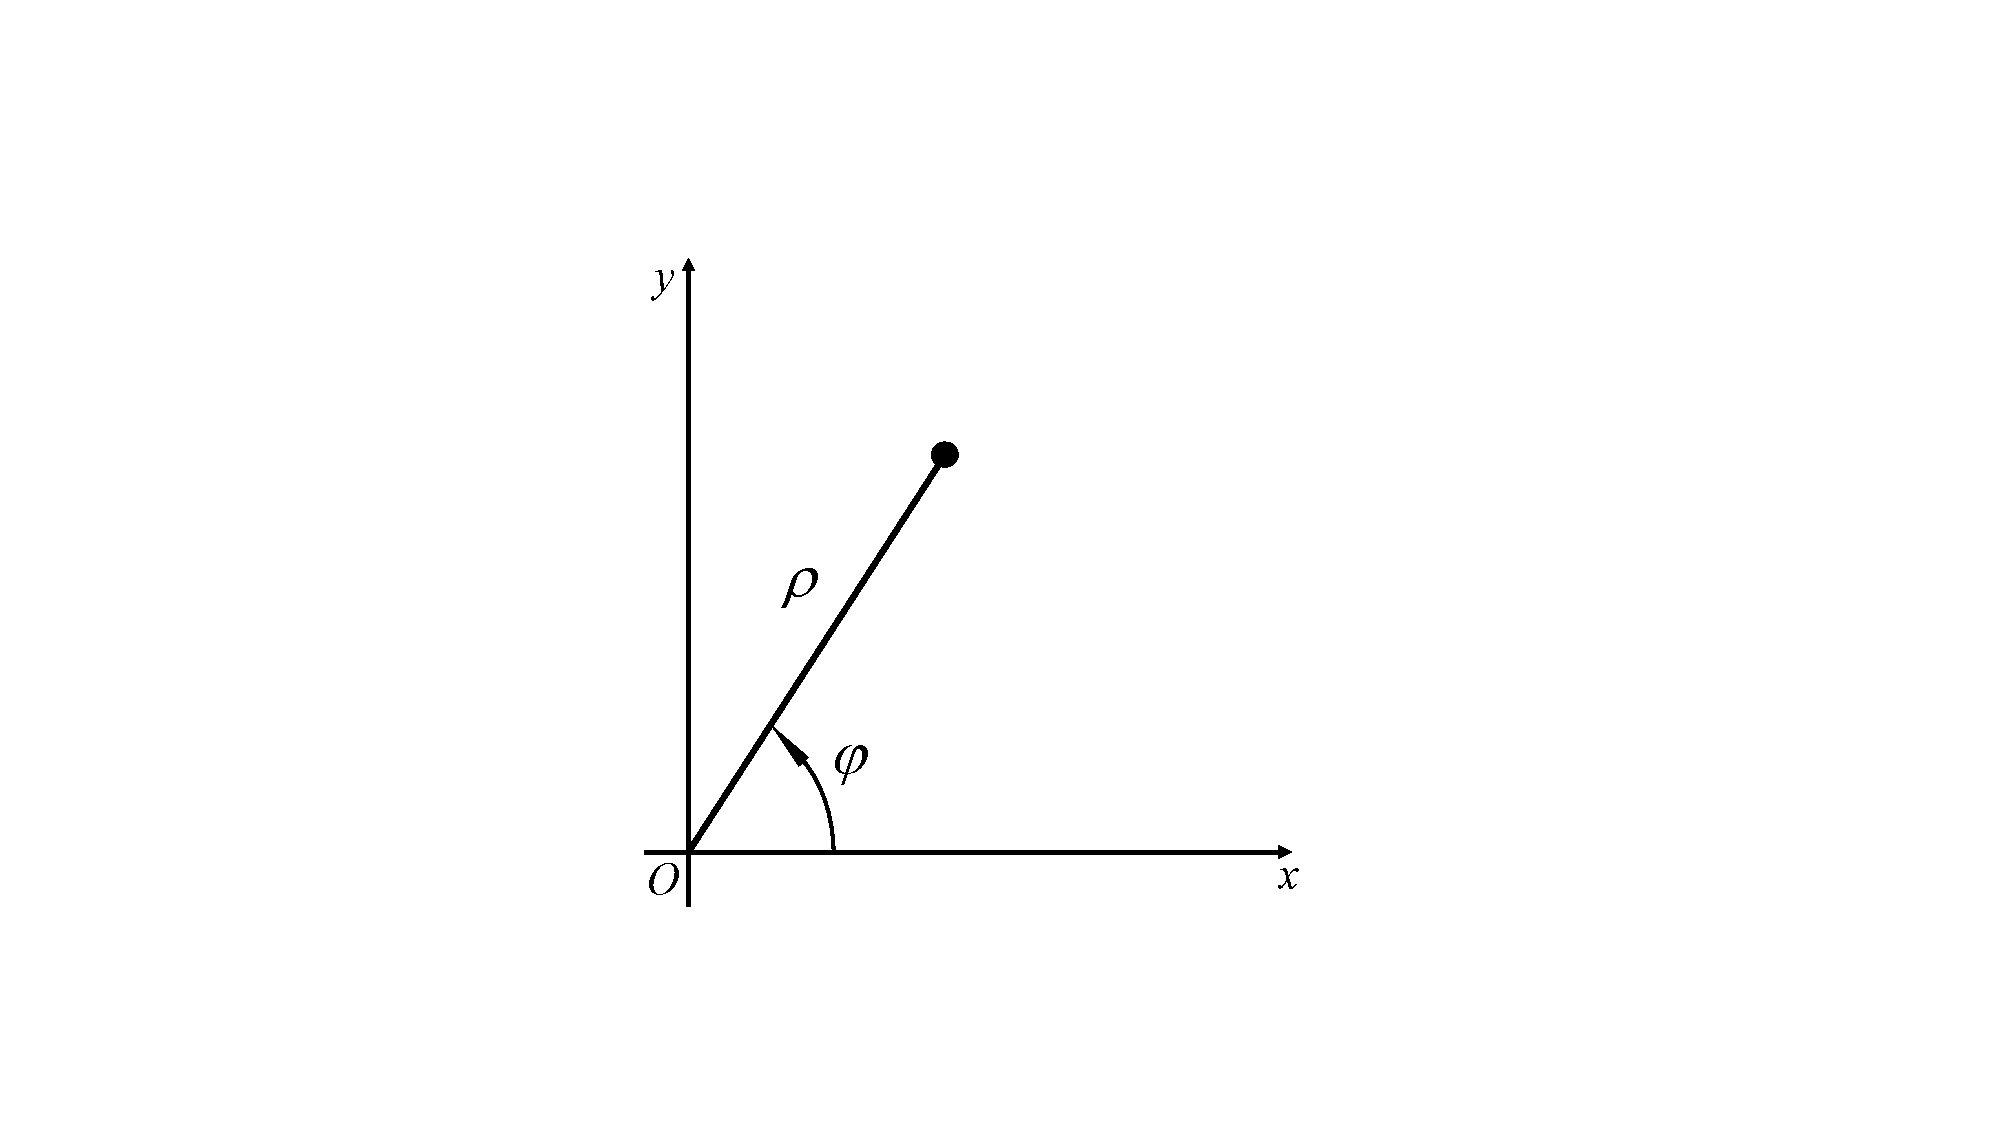
\includegraphics[width=2.5cm,clip]{QM file/figure/5-5}
	\caption{}\label{fig.5-5}
\end{wrapfigure}
\noindent 其中\eqllong
\begin{empheq}{align}\label{eq55.4}
	\nabla^{2}&=\frac{\partial^{2}}{\partial x^{2}}+\frac{\partial^{2}}{\partial y^{2}}	\nonumber\\
	&=\frac{\partial^{2}}{\partial \rho^{2}}+\frac{1}{\rho}\frac{\partial}{\partial \rho}+\frac{1}{\rho^{2}}\frac{\partial^{2}}{\partial \varphi^{2}}
\end{empheq}
角动量算符为
\begin{empheq}{equation}\label{eq55.5}
	\hat{L}_{z}=x\hat{p}_{y}-y\hat{p}_{x}=-i\hbar\frac{\partial}{\partial \varphi}
\end{empheq}\eqnormal
显然,$[\hat{L}_{z},\hat{H}]=0$,$\hat{L}_{z}$为守恒量.$\hat{H},\hat{L}_{z}$的共同本征函数可以表示成
\begin{empheq}{equation}\label{eq55.6}
	\psi(\rho,\varphi)=W(\rho)e^{im\varphi},\quad m=0,\pm1,\pm2,\cdots
\end{empheq}
$\hat{L}_{z}$的本征值为$m\hbar$.将\eqref{eq55.6}式代入能量本征方程
\eqshort
\begin{empheq}{equation}\label{eq55.7}
	\hat{H}\psi=E\psi
\end{empheq}\eqnormal
易得径向方程为
\eqllong
\begin{empheq}{equation}\label{eq55.8}
	\bigg[-\frac{\hbar^{2}}{2\mu}\bigg(\frac{d^{2}}{d\rho^{2}}+\frac{1}{\rho}\frac{d}{d\rho}\bigg)+\frac{m^{2}\hbar^{2}}{2\mu\rho^{2}}+V(\rho)\bigg]W(\rho)=EW(\rho)
\end{empheq}\eqnormal
方括号中第一项可以解释成径向动能算符,第二项为离心势能.令
\eqshort
\begin{empheq}{equation}\label{eq55.9}
	W(\rho)=\rho^{-\frac{1}{2}}v(\rho)
\end{empheq}\eqnormal
可得$v(\rho)$满足的方程为
\eqlong
\begin{empheq}{equation}\label{eq55.10}
	\bigg[-\frac{\hbar^{2}}{2\mu}\frac{d^{2}}{d\rho^{2}}+\bigg(m^{2}-\frac{1}{4}\bigg)\frac{\hbar^{2}}{2\mu\rho^{2}}+V(\rho)	\bigg]v(\rho)=Ev(\rho)
\end{empheq}\eqnormal
径向波函数及能级$E$原则上可从\eqref{eq55.8}式或\eqref{eq55.10}式解出.

\eqref{eq55.10}式的构造与三维中心力场的径向方程[\eqref{eq51.14}式]有着高度的相似性,其对应关系为
\eqindent{7}
\begin{empheq}{alignat=6}\label{eq55.11}
	\text{三维} &\quad r &\quad V(r) &\quad u(r) & l &&\quad E 	\nonumber\\
	\text{二维} &\quad \rho &\quad V(\rho) &\quad v(\rho) \quad |m|&-\frac{1}{2} &&\quad E 
\end{empheq}\eqnormal
因此,如已求得三维中心力问题的解,根据对应关系就可以写出二维中心力问题的解.反之亦然.就能级而言,在三维问题的能级公式中,将$l$换成$|m|-\frac{1}{2}$,就得到相应的二维问题能级公式.由于$l$只取正整数或0,而$|m|-\frac{1}{2}$则是半奇数,所以两种能级是不相同的.这一点和经典力学有着根本概念上的不同.在经典力学中,粒子在中心力场中运动时,其轨迹是一条平面曲线,因此,就轨道形状和能量而言,三维问题与二维问题的结果必然相同.

\example 求二维类氢离子的束缚态$(E<0)$能级.

\solution 二维类氢离子中,电子所受作用势为
\begin{empheq}{equation}\label{eq55.12}
	V(\rho)=-\frac{Z\e^{2}}{\rho}
\end{empheq}
按照上述一般理论,$\hat{H},\hat{L}_{z}$的共同本征函数可以写成
\begin{empheq}{equation}\label{eq55.13}
	\varPsi=\rho^{-1/2}v(\rho)e^{im\varphi},\quad m=0,\pm1,\pm2,\cdots
\end{empheq}
将三维类氢离子能级公式[\eqref{eq54.20}式]中$l$换成$|m|-\frac{1}{2}$,$n_{r}$改写成$n_{\rho}$(径向量子数),即得本题所求能级为
\eqlong
\begin{empheq}{equation}\label{eq55.14}
	E=\frac{Z^{2}\e^{2}}{2a_{0}\bigg(n_{\rho}+|m|+\frac{1}{2}\bigg)},\quad n_{\rho}=0,1,2,\cdots
\end{empheq}\eqnormal
其中$a_{0}=\dfrac{\hbar^{2}}{\mu \e^{2}}$(玻尔半径),就能级序列而言,相当于三维能级公式中$n\rightarrow\bigg(n-\frac{1}{2}\bigg)$.

\newpage



